\section{Desarrollo: Caso 2, configuración VFA-CFA}
\label{sec:desarrollo_c2}

\subsection{Diseño}
\label{sec:diseno_c2}

El compuesto combina el LM324 como $A_{01}$ (VFA), que aporta la precisión en continua, con el LM6181 como $A_{02}$ (CFA), que aporta la velocidad. Ambos operan en configuración no inversora y el CFA queda dentro del lazo global: la ganancia total la fija la red $R_i$--$R_f$ y la ganancia local del CFA, $A_{vfi2}$, la red $R_1$--$R_2$. Se busca un ancho de banda potencial $f_g \approx \SI{2}{MHz}$ con una respuesta cercana a MPM, teniendo en cuenta el segundo polo del VFA.

\paragraph{Ganancia del CFA.} Según la \autoref{sec:compuesto_distinto}, el ancho de banda potencial fija la ganancia local del CFA (\autoref{eq:wg_VFACFA}), y la condición de MPM impone una cota superior (\autoref{eq:Avfi2_max}):
\begin{gather}
    A_{vfi2} = \frac{f_g}{K\,f_T} = \frac{\SI{2}{MHz}}{0{,}1\cdot\SI{1}{MHz}} = 20 \\
    A_{vfi2,max} = \frac{f_2}{2\,K\,f_T} = \frac{\SI{5,06}{MHz}}{2\cdot 0{,}1\cdot\SI{1}{MHz}} = 25{,}3
\end{gather}
Se adopta $A_{vfi2} = 20 < A_{vfi2,max}$. Con este valor $Q_p^2 = f_g/f_2 = 0{,}395$ (\autoref{eq:Qp_VFACFA}), es decir, una respuesta algo más amortiguada que MPM ($Q_p^2 = 1/2$), lo que deja margen para el atraso de fase que agregan los polos del CFA.

\paragraph{Red local del CFA.} Se toma $R_2 = \SI{820}{\ohm}$ (valor recomendado por el fabricante) y $r_i = \SI{20}{\ohm}$ (supuesto, pues el fabricante no lo publica). Resulta
\begin{gather}
    R_1 = \frac{R_2}{A_{vfi2}-1} = \frac{820}{19} = \SI{43,16}{\ohm} \\
    R_{eff} = R_2 + r_i\,A_{vfi2} = 820 + 20\cdot 20 = \SI{1220}{\ohm} \\
    f_{cfa} = \frac{1}{2\pi\,C_t\,R_{eff}} = \SI{27,2}{MHz}
\end{gather}
El polo del CFA queda $14$ veces por encima de $f_g$ y el margen de fase del CFA aislado es $\ang{72,5}$ (\autoref{eq:Mphi_CFA}), por lo que el valor elegido de $R_2$ es estable. La \autoref{tab:parametros_vfa_cfa} reúne el diseño completo.

\begin{table}[H]
\centering
\caption{Diseño VFA-CFA: expresiones, cálculo y valores.}
\label{tab:parametros_vfa_cfa}
\footnotesize
\setlength{\tabcolsep}{4pt}
\begin{tabular}{>{\raggedright\arraybackslash}p{0.31\textwidth} >{\centering\arraybackslash}p{0.2\textwidth} >{\centering\arraybackslash}p{0.27\textwidth} >{\centering\arraybackslash}p{0.13\textwidth}}
\toprule
\textbf{Parámetro} & \textbf{Expresión} & \textbf{Cálculo} & \textbf{Valor} \\
\midrule
Ganancia global $A_{vf}$ & dato & \SI{20}{dB} & \SI{10}{V/V} \\
Factor de realimentación $K$ & $1/A_{vf}$ & $1/10$ & \num{0,1} \\
Resistencia de entrada global $R_i$ & elegida & --- & \SI{1}{k\ohm} \\
Resistencia de realimentación global $R_f$ & $R_i(A_{vf}-1)$ & $1\text{ k}\Omega\cdot 9$ & \SI{9}{k\ohm} \\
Ganancia del CFA $A_{vfi2}$ & $f_g/(K f_T)$ & $2\text{ MHz}/(0{,}1\cdot 1\text{ MHz})$ & \SI{20}{V/V} \\
Cota de MPM $A_{vfi2,max}$ & $f_2/(2Kf_T)$ & $5{,}06\text{ MHz}/0{,}2\text{ MHz}$ & \SI{25,3}{V/V} \\
Realimentación local $R_2$ & elegida (fabricante) & --- & \SI{820}{\ohm} \\
Resistencia local a tierra $R_1$ & $R_2/(A_{vfi2}-1)$ & $820/19$ & \SI{43,16}{\ohm} \\
Resistencia efectiva $R_{eff}$ & $R_2 + r_iA_{vfi2}$ & $820 + 20\cdot 20$ & \SI{1220}{\ohm} \\
Polo del CFA $f_{cfa}$ & $1/(2\pi C_tR_{eff})$ & --- & \SI{27,2}{MHz} \\
Ganancia de lazo en continua $T_0$ & $K\,A_{d0}\,A_{vfi2}$ & $0{,}1\cdot 10^5\cdot 20$ & \num{200000} (\SI{106}{dB}) \\
Separación de polos $D_p$ & $f_2/f_1$ & $5{,}06\text{ MHz}/10\text{ Hz}$ & \num{506000} \\
\bottomrule
\end{tabular}
\end{table}

\subsection{Resultados analíticos}
\label{sec:analitico_c2}

Con $T(s)\cong T_0/[(1+s/\omega_1)(1+s/\omega_2)]$ y las relaciones de la \autoref{sec:mpm} se obtienen los valores de la \autoref{tab:analitica_c2}. Los polos de lazo cerrado son $s^2 + (\omega_1+\omega_2)s + \omega_1\omega_2(1+T_0) = 0$, y el margen de fase se calcula sobre el cruce exacto de $|T|=1$; el resultado coincide con la fórmula del apunte $M_\varphi = 90^\circ - \arctan(\Omega_GQ_p)$, que vale para cualquier $Q_p$ (\autoref{eq:omegaG}).

\begin{table}[H]
\centering
\caption{Resultados analíticos (modelo de dos polos), Caso 2.}
\label{tab:analitica_c2}
\small
\setlength{\tabcolsep}{4pt}
\begin{tabular}{>{\raggedright\arraybackslash}p{0.37\textwidth} >{\centering\arraybackslash}p{0.31\textwidth} >{\centering\arraybackslash}p{0.2\textwidth}}
\toprule
\textbf{Magnitud} & \textbf{Expresión} & \textbf{Valor} \\
\midrule
Ancho de banda potencial $f_g$ & $K\,A_{vfi2}\,f_T$ & \SI{2,000}{MHz} \\
Cruce exacto de $T$, $f_{Gc}$ & $|T(jf)|=1$ & \SI{1,875}{MHz} \\
$\Omega_G = f_{Gc}/f_p$ & --- & \num{0,5895} \\
Margen de fase $M_\varphi$ & \autoref{eq:Mphi_2polos} & \ang{69,66} \\
Frecuencia de los polos $f_p$ & $\sqrt{\omega_1\omega_2(1+T_0)}/2\pi$ & \SI{3,181}{MHz} \\
Factor de calidad $Q_p$ & $\omega_p/(\omega_1+\omega_2)$ & \num{0,629} \\
Amortiguamiento $\zeta$ & $1/(2Q_p)$ & \num{0,795} \\
Polos de lazo cerrado & $s_{1,2}$ & $(-2{,}530 \pm j\,1{,}929)$ MHz \\
Ancho de banda real $f_H$ ($-3$ dB) & $f_p\sqrt{a+\sqrt{a^2+1}}$ & \SI{2,791}{MHz} \\
\bottomrule
\end{tabular}
\end{table}

Como $Q_p<1/\sqrt2$, la respuesta es más amortiguada que MPM; el ancho de banda real ($\SI{2,79}{MHz}$) resulta mayor que el potencial ($f_g=\SI{2}{MHz}$), igual que en el Caso 1.

Para incluir el efecto del CFA se armó el modelo de cuatro polos, con el CFA realimentado de la \autoref{eq:Avf_CFA_ri} y $Z_t$ de dos polos. Sus resultados se comparan en la \autoref{tab:modelos_c2}. El CFA agrega atraso de fase, por lo que el margen de fase baja respecto del modelo simple, y eleva el $Q_p$ y el ancho de banda.

\begin{table}[H]
\centering
\caption{Resultados numéricos: modelo de 2 polos y de 4 polos, Caso 2.}
\label{tab:modelos_c2}
\begin{tabular}{lcc}
\toprule
\textbf{Magnitud} & \textbf{2 polos} & \textbf{4 polos} \\
\midrule
Frecuencia crítica $f_{Gc}$ [MHz] & 1,875 & 1,873 \\
Margen de fase [$^\circ$] & 69,66 & 65,74 \\
Margen de ganancia [dB] & $\infty$ & 23,2 \\
Ancho de banda real ($-3$ dB) [MHz] & 2,791 & 3,039 \\
Frecuencia de los polos $f_p$ [MHz] & 3,181 & 3,165 \\
Factor de calidad $Q_p$ & 0,629 & 0,681 \\
Polos dominantes [MHz] & $-2{,}530 \pm j\,1{,}929$ & $-2{,}322 \pm j\,2{,}150$ \\
\bottomrule
\end{tabular}
\end{table}

\emph{Nota:} el margen de ganancia del modelo de dos polos es infinito porque la fase de $T(s)$ tiende asintóticamente a $-180^\circ$ sin alcanzarlo a ninguna frecuencia finita; con cuatro polos la fase sí cruza $-180^\circ$ y el margen de ganancia es finito.

\begin{figure}[H]
    \centering
    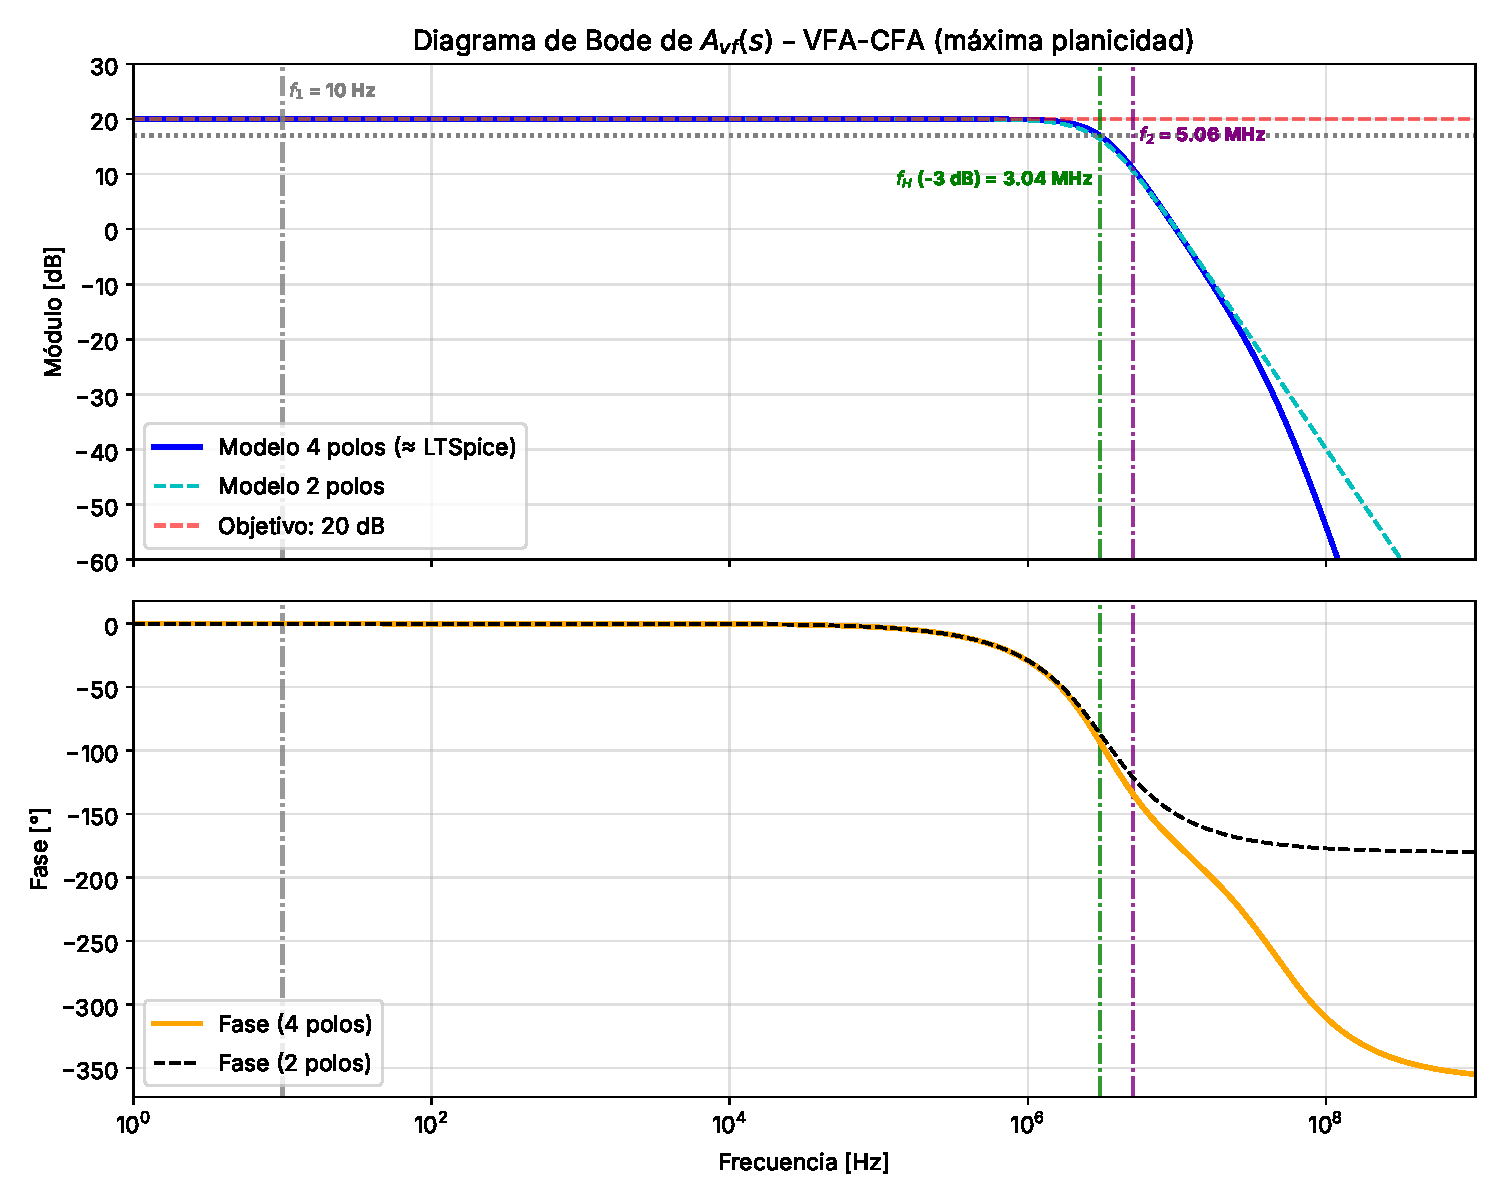
\includegraphics[width=0.95\linewidth,height=0.42\textheight,keepaspectratio]{Imagenes/c2_bode_lazo_cerrado.pdf}
    \caption{Diagrama de Bode a lazo cerrado (modelos de 2 y 4 polos), Caso 2.}
    \label{fig:bode_lc_c2}
\end{figure}

\begin{figure}[H]
    \centering
    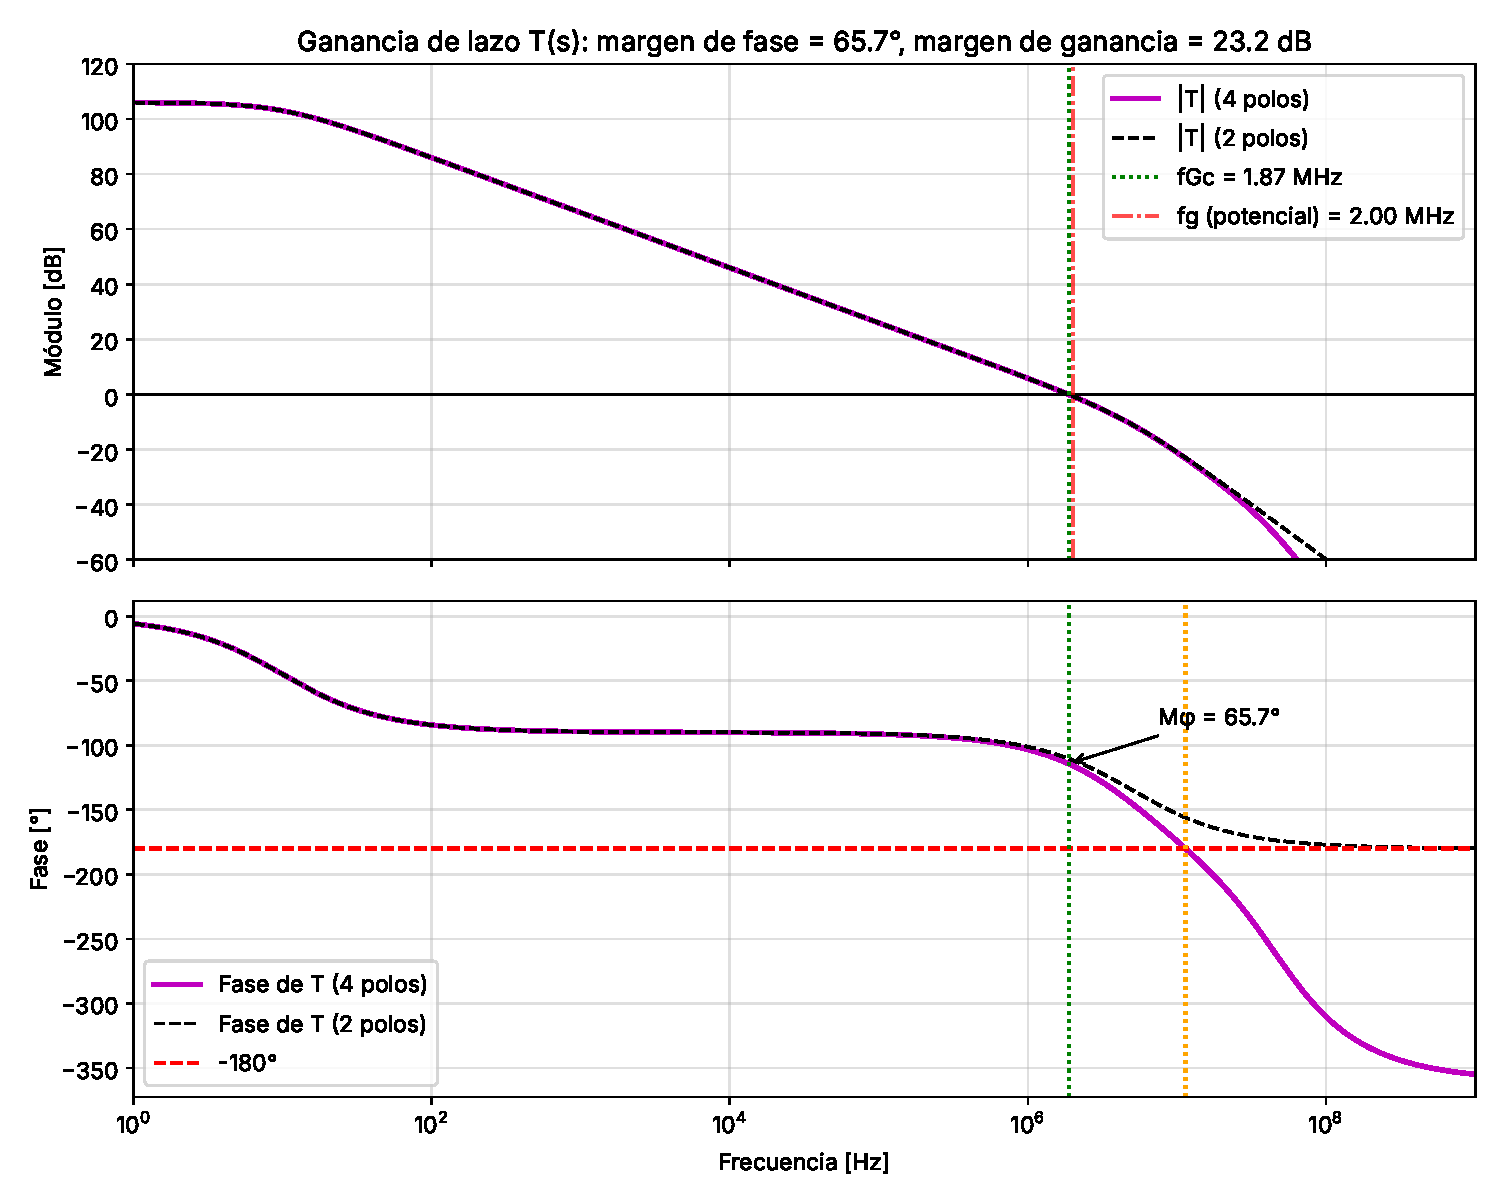
\includegraphics[width=0.95\linewidth,height=0.42\textheight,keepaspectratio]{Imagenes/c2_bode_ganancia_lazo.pdf}
    \caption{Diagrama de Bode de la ganancia de lazo, Caso 2: frecuencia crítica y margen de fase.}
    \label{fig:bode_lazo_c2}
\end{figure}

\paragraph{Sensibilidad al valor de $r_i$.} Como $r_i$ no está publicado, se repitió el modelo de cuatro polos para distintos valores (\autoref{tab:ri_c2}). El margen de fase varía menos de $3^\circ$ entre $r_i\approx0$ y $\SI{50}{\ohm}$, por lo que el supuesto no es crítico.

\begin{table}[H]
\centering
\caption{Sensibilidad al valor de $r_i$ (modelo de 4 polos), Caso 2.}
\label{tab:ri_c2}
\begin{tabular}{cccccc}
\toprule
$r_i$ [$\Omega$] & $R_{eff}$ [$\Omega$] & $f_{Gc}$ [MHz] & $M_\varphi$ [$^\circ$] & $M_G$ [dB] & BW [MHz] \\
\midrule
0 & 820 & 1,875 & 67,0 & 26,2 & 2,962 \\
10 & 1020 & 1,874 & 66,4 & 24,5 & 3,001 \\
20 & 1220 & 1,873 & 65,7 & 23,2 & 3,039 \\
30 & 1420 & 1,872 & 65,1 & 22,1 & 3,075 \\
50 & 1820 & 1,869 & 63,9 & 20,4 & 3,142 \\
\bottomrule
\end{tabular}
\end{table}

\paragraph{Respuesta al escalón teórica.} La \autoref{fig:escalon_teorico_c2} muestra la respuesta a un escalón de $\SI{0,1}{V}$ (salida de $\SI{1}{V}$) de los modelos de dos y de cuatro polos; los valores de sobrepico y margen de fase estimado se comparan con la simulación en la \autoref{tab:escalon_c2}.

\begin{figure}[H]
    \centering
    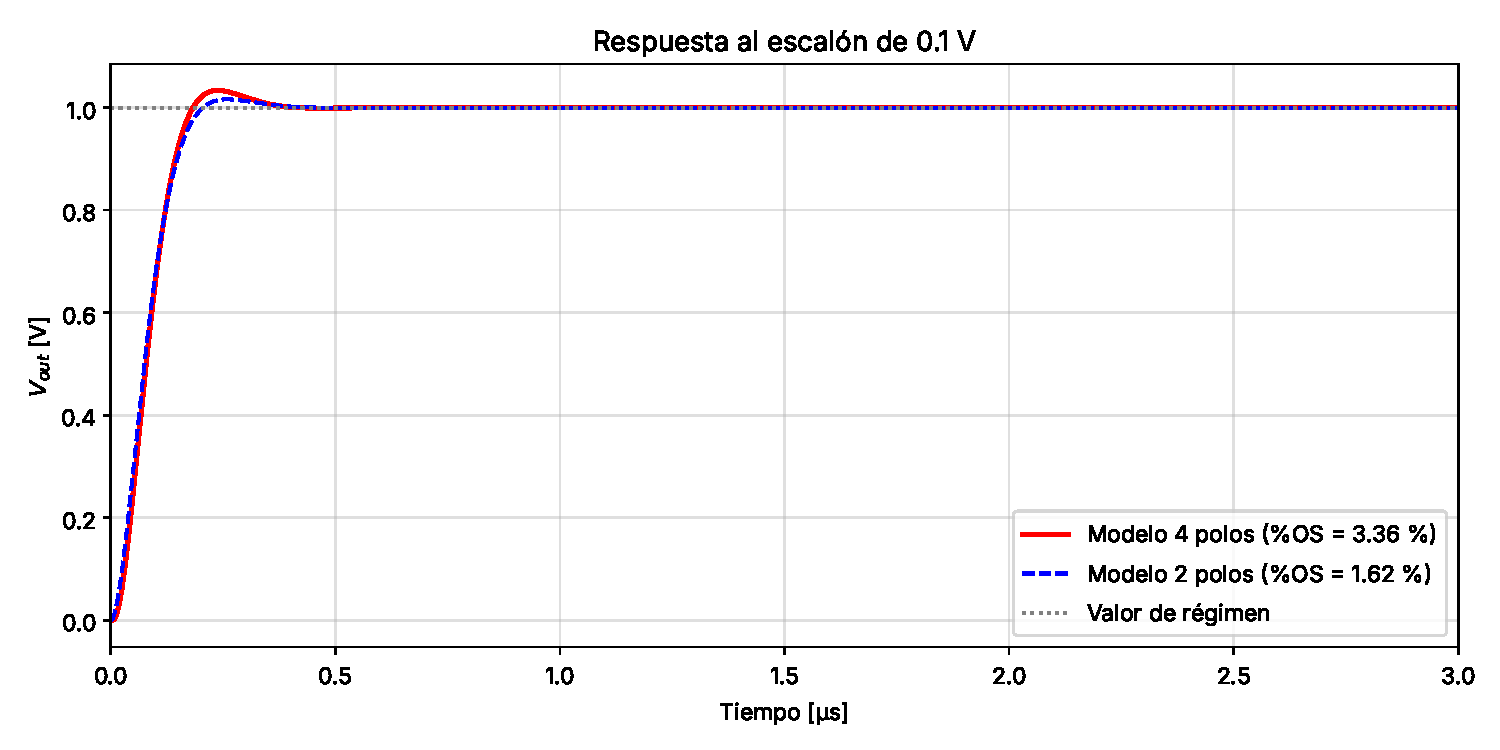
\includegraphics[width=0.95\linewidth,height=0.42\textheight,keepaspectratio]{Imagenes/c2_escalon_teorico.pdf}
    \caption{Respuesta al escalón teórica (2 y 4 polos), Caso 2.}
    \label{fig:escalon_teorico_c2}
\end{figure}

\subsection{Simulación}
\label{sec:simulacion_c2}

Se simularon en LTSpice los circuitos de lazo abierto, ganancia de lazo y lazo cerrado del compuesto VFA-CFA, con los modelos del LM324 (con la etapa de salida de adaptación de impedancia) y del LM6181. El esquemático usa $R_i = \SI{1}{k\ohm}$, $R_f = \SI{9}{k\ohm}$, $R_2 = \SI{820}{\ohm}$ y $R_1 = \SI{43,2}{\ohm}$.

\begin{figure}[H]
    \centering
    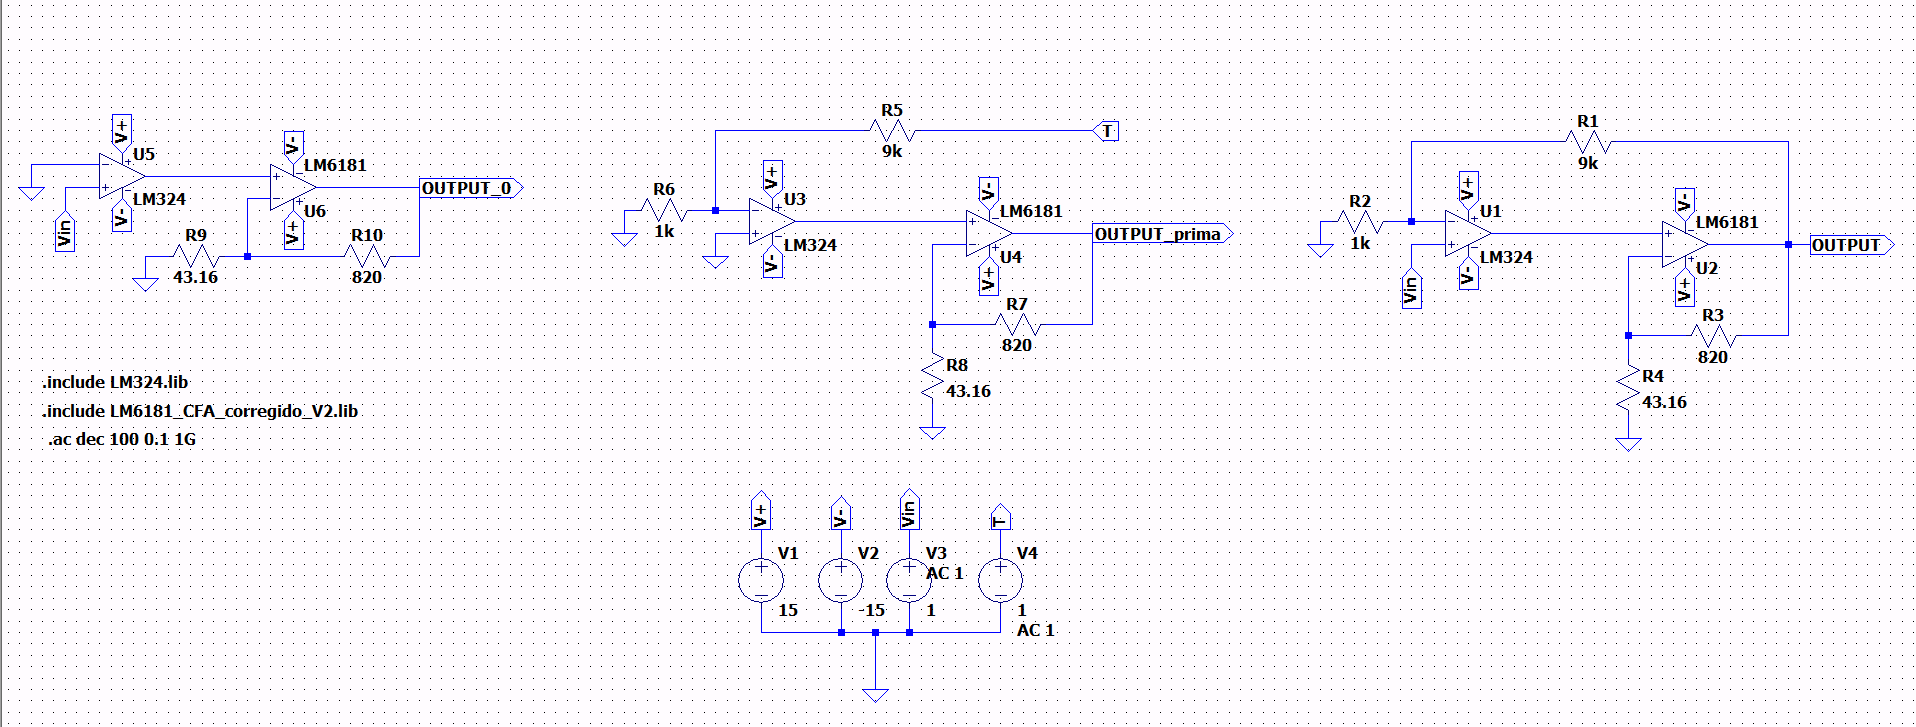
\includegraphics[width=1.0\linewidth,height=0.32\textheight,keepaspectratio]{Imagenes/c2_sim_circuitos.png}
    \caption{Esquemático VFA-CFA en LTSpice: lazo abierto (izquierda), ganancia de lazo (centro) y lazo cerrado (derecha).}
    \label{fig:circuito_VFA_CFA}
\end{figure}

\subsubsection{Respuesta en frecuencia a lazo abierto}
La \autoref{fig:rta_frec_open_loop_c2} muestra una ganancia en banda media de $A_{d0}A_{vfi2} = 100\text{ dB} + 26\text{ dB} = 126\text{ dB}$, con el primer polo en $f_1=\SI{10}{Hz}$ y pendiente $-20$ dB/dec hasta que actúan el segundo polo del VFA ($f_2$) y los del CFA.

\begin{figure}[H]
    \centering
    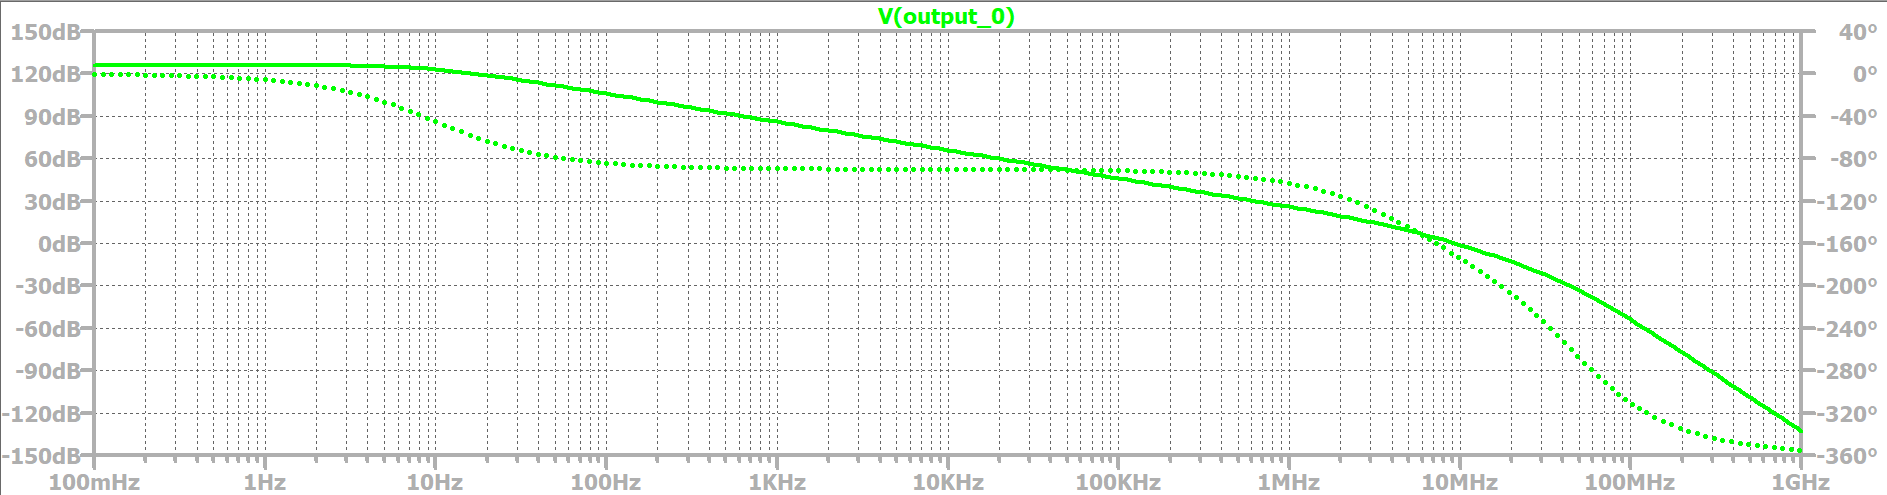
\includegraphics[width=0.95\linewidth,height=0.32\textheight,keepaspectratio]{Imagenes/c2_sim_lazo_abierto.png}
    \caption{Respuesta en frecuencia a \textbf{lazo abierto} del compuesto (módulo y fase).}
    \label{fig:rta_frec_open_loop_c2}
\end{figure}

\subsubsection{Respuesta en frecuencia de la ganancia de lazo}
Con los cursores sobre la curva de $-T$ (\texttt{V(output\_prima)}) se midió el cruce por \SI{0}{dB} en $f_{Gc} = \SI{1,873}{MHz}$, donde la fase es $M_\varphi = \ang{65,78}$ (el modelo de 4 polos predice \SI{1,873}{MHz} y \ang{65,74}). La ganancia de lazo en continua es de \SI{106}{dB}, con el polo dominante en \SI{10}{Hz}, y la curva a lazo abierto del compuesto (\texttt{V(output\_0)}) da \SI{126}{dB}, es decir $T_0 + 20\,\mathrm{dB}$, como corresponde a $T = K\,A$.

\begin{figure}[H]
    \centering
    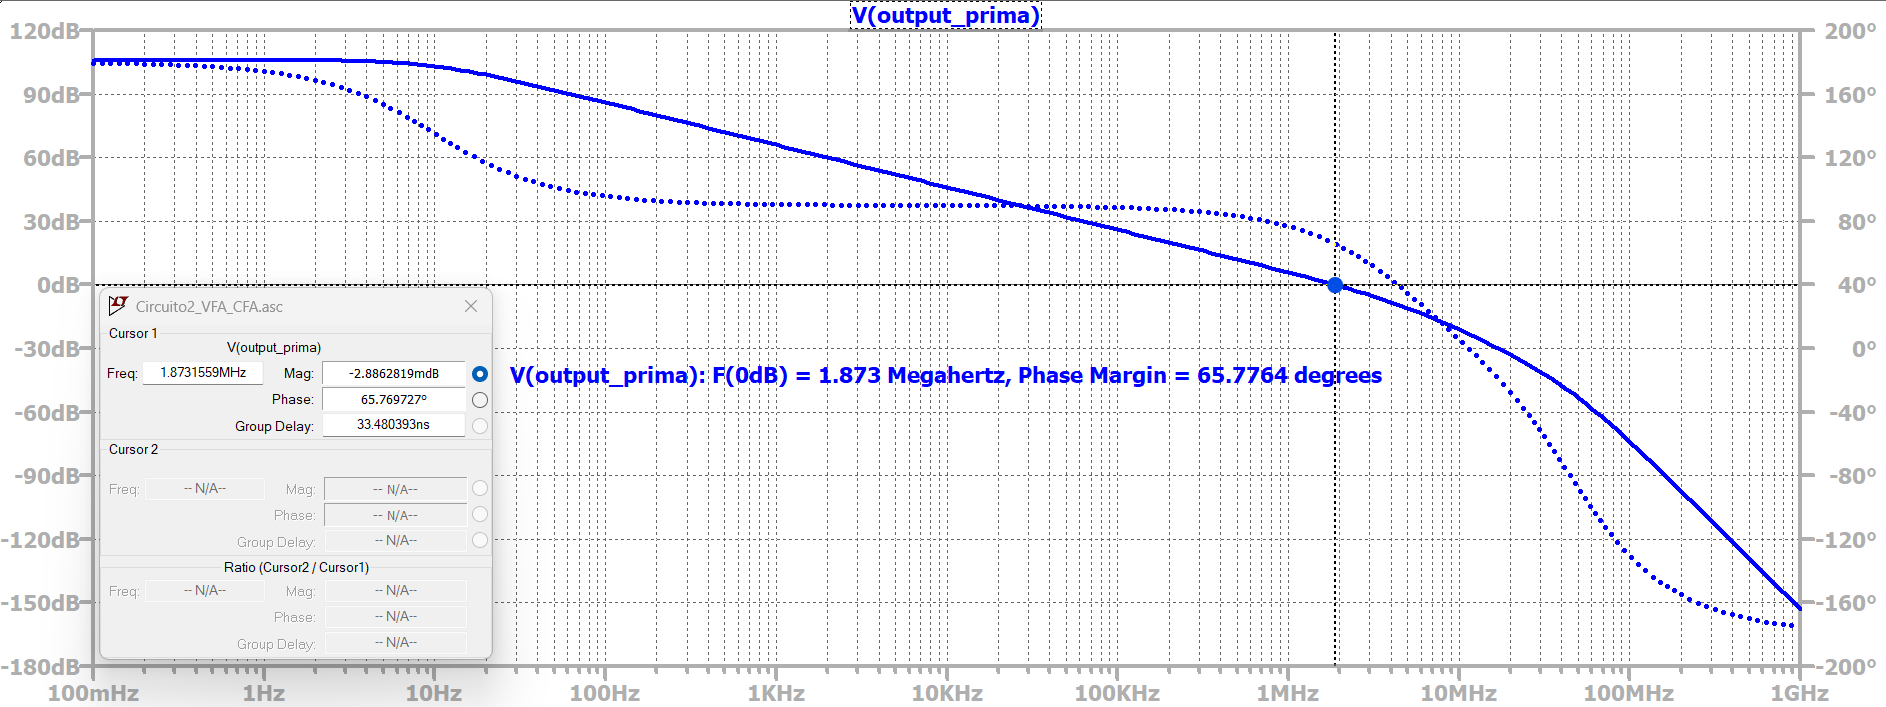
\includegraphics[width=0.95\linewidth,height=0.32\textheight,keepaspectratio]{Imagenes/c2_sim_lazo_T.png}
    \caption{Respuesta en frecuencia de la \textbf{ganancia de lazo} ($-T$): $f_{Gc} = \SI{1,873}{MHz}$ y $M_\varphi = \ang{65,78}$.}
    \label{fig:rta_frec_loop_c2}
\end{figure}

\subsubsection{Respuesta en frecuencia a lazo cerrado}
La \autoref{fig:rta_frec_close_loop_c2} confirma la ganancia en banda media de $\SI{20}{dB}$ ($\SI{19,9999}{dB}$ a $\SI{38,8}{kHz}$), sin sobrepico. Con el cursor a $\SI{17}{dB}$ se obtuvo $\SI{16,949}{dB}$ a $\SI{3,052}{MHz}$ ($-3{,}05$ dB respecto de banda media); interpolando al punto de $-3{,}01$ dB resulta un ancho de banda real $f_H \approx \SI{3,04}{MHz}$ (el modelo de cuatro polos predice $\SI{3,039}{MHz}$).

\begin{figure}[H]
    \centering
    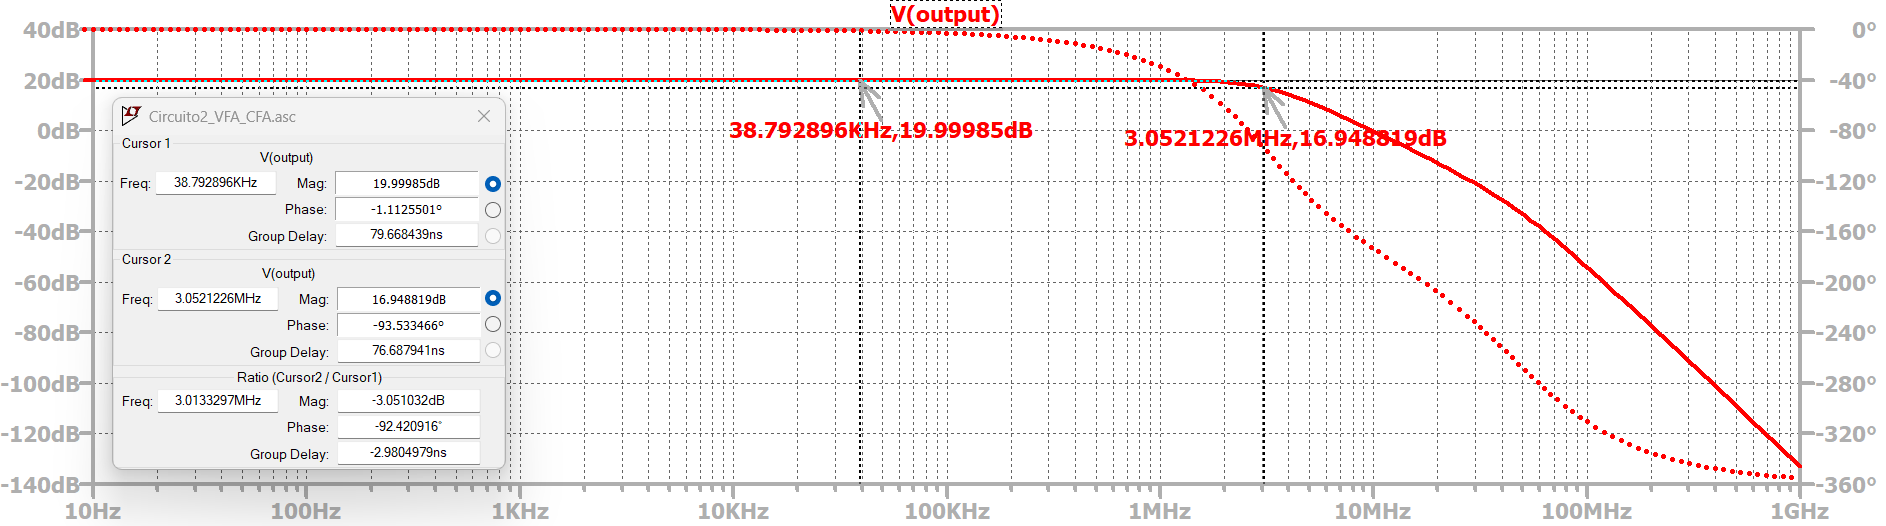
\includegraphics[width=0.95\linewidth,height=0.32\textheight,keepaspectratio]{Imagenes/c2_sim_lazo_cerrado.png}
    \caption{Respuesta en frecuencia a \textbf{lazo cerrado}.}
    \label{fig:rta_frec_close_loop_c2}
\end{figure}

\subsubsection{Respuesta al escalón}
Se aplica un escalón de $\SI{0,1}{V}$ (salida de $\SI{1}{V}$) para trabajar en pequeña señal y evitar que el \emph{slew rate} distorsione el sobrepico. El modelo de cuatro polos predice $\mathrm{\char37}OS = 3{,}36\,\mathrm{\char37}$. En la simulación se midió $V_{pico} = \SI{1,0333}{V}$ (a \SI{251}{ns}, \SI{241}{ns} después del escalón) y $V_{est} = \SI{0,9998}{V}$, de donde
\begin{gather}
    \mathrm{\char37}OS = \frac{1{,}0333 - 0{,}9998}{0{,}9998}\cdot 100 = 3{,}35\,\mathrm{\char37} \\
    \zeta = \frac{-\ln(0{,}0335)}{\sqrt{\pi^2+\ln^2(0{,}0335)}} = 0{,}734 \qquad MF \approx \ang{66,9}
\end{gather}
(\autoref{tab:escalon_c2}).



\begin{figure}[H]
    \centering
    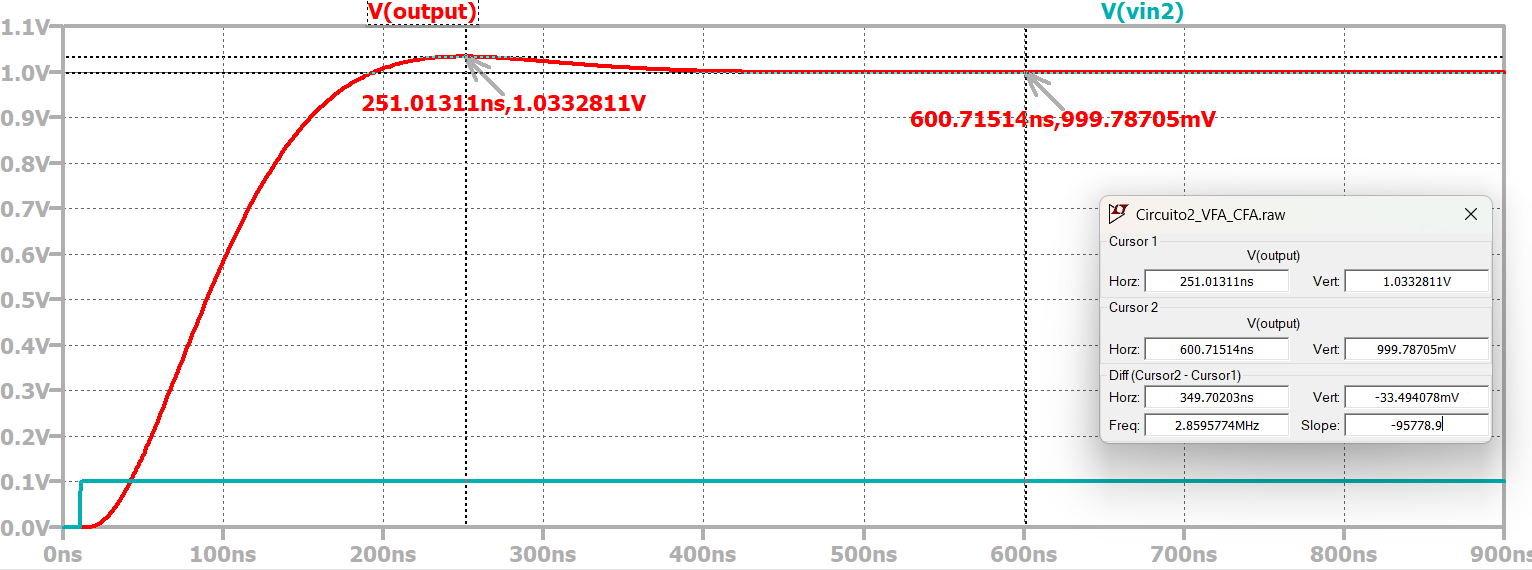
\includegraphics[width=0.95\linewidth,height=0.32\textheight,keepaspectratio]{Imagenes/c2_sim_escalon.png}
    \caption{Respuesta al escalón de $\SI{0,1}{V}$ (LTSpice): $V_{pico} = \SI{1,0333}{V}$ y $V_{est} = \SI{0,9998}{V}$.}
    \label{fig:rta_step_c2}
\end{figure}

\subsection{Comparación de resultados}
\label{sec:comparacion_c2}

\begin{table}[H]
\centering
\caption{Comparación entre teoría y simulación (VFA-CFA). Error $= (\text{teórico}-\text{LTSpice})/\text{LTSpice}$.}
\label{tab:final_c2}
\small
\setlength{\tabcolsep}{4pt}
\begin{tabularx}{\textwidth}{>{\raggedright\arraybackslash}X c c c c c}
\toprule
\textbf{Magnitud} & \textbf{Analítico} & \textbf{4 polos} & \textbf{LTSpice} & \textbf{Err. anal. [\%]} & \textbf{Err. 4p [\%]} \\
\midrule
Ancho de banda potencial $f_g$ [MHz] & 2,000 & --- & --- & --- & --- \\
Cruce de $T$ exacto $f_{Gc}$ [MHz] & 1,875 & 1,873 & 1,873 & $+0{,}1$ & $0{,}0$ \\
Margen de fase del lazo [$^\circ$] & 69,66 & 65,74 & 65,78 & $+5{,}9$ & $-0{,}1$ \\
Frecuencia de polos $f_p$ [MHz] & 3,181 & 3,165 & --- & --- & --- \\
Ancho de banda real $f_H$ [MHz] & 2,791 & 3,039 & 3,04 & $-8{,}1$ & $+0{,}1$ \\
Sobrepico \%OS [\%] & 1,62 & 3,36 & 3,35 & $-51{,}6$ & $+0{,}2$ \\
$M_\varphi$ desde el escalón [$^\circ$] & 69,66 & 66,88 & 66,89 & $+4{,}1$ & $0{,}0$ \\
\bottomrule
\end{tabularx}
\end{table}

\begin{table}[H]
\centering
\caption{Respuesta al escalón y margen de fase estimado, Caso 2.}
\label{tab:escalon_c2}
\begin{tabular}{lccc}
\toprule
\textbf{Magnitud} & \textbf{2 polos} & \textbf{4 polos} & \textbf{LTSpice} \\
\midrule
$V_{pico}$ [V] & 1,0162 & 1,0336 & 1,0333 \\
$V_{est}$ [V] & 1,0000 & 1,0000 & 0,9998 \\
$\mathrm{\char37}OS$ & 1,62 & 3,36 & 3,35 \\
$\zeta$ & 0,7953 & 0,7339 & 0,7341 \\
$M_\varphi$ estimado [$^\circ$] & 69,66 & 66,88 & 66,89 \\
\bottomrule
\end{tabular}
\end{table}

\subsection{Análisis y conclusión parcial}
\label{sec:concl_c2}

\begin{itemize}
    \item El diseño logra un ancho de banda potencial $f_g = K\,A_{vfi2}\,f_T = \SI{2}{MHz}$, unas $6{,}3$ veces el del compuesto VFA-VFA del Caso 1 ($\SI{316}{kHz}$), porque el CFA aporta ganancia local $A_{vfi2}=20$ sin perder ancho de banda. El cruce real de la ganancia de lazo ($f_{Gc} = \SI{1,87}{MHz}$ medido) queda por debajo de $f_g$ porque $f_g$ es el cruce asintótico; aun así es $\approx9$ veces el del Caso 1 ($\SI{206}{kHz}$).
    \item El ancho de banda real previsto ($\approx\SI{3}{MHz}$) supera a $f_g$, como en el Caso 1, porque con $Q_p\approx0{,}63$ a $0{,}68$ la respuesta es plana y la frecuencia de los polos ($f_p\approx\SI{3,2}{MHz}$) está por encima del cruce de $T$.
    \item El modelo de dos polos sobreestima el margen de fase en $\approx4^\circ$ ($69{,}7^\circ$ contra $65{,}7^\circ$) porque desprecia el atraso de fase de los polos del CFA. La tabla de sensibilidad muestra que el supuesto de $r_i$ modifica el margen de fase en menos de $3^\circ$.
    \item El valor de $A_{vfi2}$ se eligió por debajo de la cota de MPM ($25{,}3$), con la que el margen de fase del modelo de cuatro polos sería del orden de $60^\circ$ y habría pico en el módulo.
    \item La simulación coincide con el modelo de cuatro polos con errores menores al $0{,}2\,\mathrm{\char37}$ en $f_{Gc}$, margen de fase y sobrepico, lo que valida el modelo del CFA realimentado (\autoref{eq:Avf_CFA_ri}). El modelo de dos polos queda $\approx 4^\circ$ por encima en el margen de fase y predice la mitad del sobrepico.
    \item El margen de fase estimado a partir del escalón ($\ang{66,9}$) difiere en $\approx1^\circ$ del medido en el lazo ($\ang{65,8}$), diferencia esperable porque la relación entre sobrepico y margen de fase es exacta solo para segundo orden y aquí el sistema tiene cuatro polos.
    \item El ancho de banda real medido ($\approx\SI{3,04}{MHz}$) coincide con el modelo de cuatro polos y es $\approx8\,\mathrm{\char37}$ mayor que el del modelo de dos polos ($\SI{2,79}{MHz}$); ambos superan al potencial $f_g = \SI{2}{MHz}$ porque con $Q_p\approx0{,}68$ la respuesta es plana y $f_p>f_g$. No se observa pico en el módulo, como se esperaba para $Q_p<1/\sqrt2$ (apenas por debajo de MPM en el modelo simple).
    \item En conjunto, el compuesto VFA-CFA cumple los requerimientos: ganancia de $\SI{20}{dB}$, ancho de banda real de $\SI{3,04}{MHz}$ (frente a $\SI{345}{kHz}$ del compuesto VFA-VFA del Caso 1, casi $9$ veces mayor) y margen de fase de $\ang{65,8}$, equivalente al de MPM.
\end{itemize}
